\documentclass[12pt]{article}
\usepackage[a4paper,left=2.5cm,right=2.5cm,top=2.5cm,bottom=2.5cm]{geometry}
%\usepackage[margin=0.5in]{geometry}
\usepackage[utf8]{inputenc}
\usepackage{graphicx}
\usepackage{float}
\usepackage{multicol}
\usepackage{wrapfig}
\usepackage{multirow}
\usepackage{subcaption}
\graphicspath{ {images/} }




\begin{document}



\begin{titlepage}

\newcommand{\HRule}{\rule{\linewidth}{0.5mm}} % Defines a new command for the horizontal lines, change thickness hereru

\center % Center everything on the page
 
%----------------------------------------------------------------------------------------
%	HEADING SECTIONS
%----------------------------------------------------------------------------------------

\textsc{\LARGE Tata Institute of Fundamental Research}\\[1.5cm] 
%\textsc{\Large TIFR Graduate School Project Report, June 2018}\\[0.5cm] % Major heading such as course name
\textsc{\large Graduate School Project Report}\\[0.5cm] % Minor heading such as course title
\vspace{4cm}
%----------------------------------------------------------------------------------------
%	TITLE SECTION
%----------------------------------------------------------------------------------------

\HRule \\[0.4cm]
{ \huge \bfseries Comparison of CORSIKA Hadronic Interaction Models}\\[0.4cm] % Title of your document
\HRule \\[1.5cm]
 
%----------------------------------------------------------------------------------------
%	AUTHOR SECTION
%----------------------------------------------------------------------------------------

\vspace{4cm}

\begin{minipage}{0.4\textwidth}
\begin{flushleft} \large
\emph{Author:}\\
Mohit Saharan\\
DHEP, TIFR, Mumbai
% Your name
\end{flushleft}
\end{minipage}
~
\begin{minipage}{0.4\textwidth}
\begin{flushright} \large
\emph{Supervisor:} \\
Dr. Pravata K. Mohanty\\
DHEP, TIFR, Mumbai
\end{flushright}
\end{minipage}\\[2cm]

% If you don't want a supervisor, uncomment the two lines below and remove the section above
%\Large \emph{Author:}\\
%John \textsc{Smith}\\[3cm] % Your name

%----------------------------------------------------------------------------------------
%	DATE SECTION
%----------------------------------------------------------------------------------------

{\large \today}\\[2cm] % Date, change the \today to a set date if you want to be precise

%----------------------------------------------------------------------------------------
%	LOGO SECTION
%----------------------------------------------------------------------------------------

%\includegraphics{tifr_logo.png}\\[1cm] % Include a department/university logo - this will require the graphicx package
 
%----------------------------------------------------------------------------------------

\vfill % Fill the rest of the page with whitespace

\end{titlepage}
\pagebreak


\begin{abstract}
In GRAPES-3 experiment, hadronic interaction generators of CORSIKA simulation program are used to derive the energy and composition of primary cosmic rays (PCRs). The results are highly dependent on the assumptions taken by different type of  generators. This study compares the two generators from CORSIKA-7.69: SIBYLL-2.3c and QGSJETII-04, on the basis of muon multiplicity distributions(MMDs). The parameters of SIBYLL-2.3c and QGSJETII-04 are tuned to LHC data and hence are called post-LHC generators. Low energy hadronic interactions were treated by FLUKA-2011. In this study, MMDs of monoenenergetic showers with zenith angle $theta$ = 0$^\circ$, induced by H, He, N, Al, and Fe primary at energies$-$10 TeV, 100 TeV, and 1000 TeV were compared. MMDs of monoenergetic proton (H) initiated showers simulated using post-LHC generators were  also compared with that of pre-LHC generators (SIBYLL-2.1 and QGSJETII-03 of CORSIKA-6.99). Proton initiated showers with primary energy $10^{13} eV < $ E $<10^{15}$ eV, and zenith angle$0^\circ<\theta<60^\circ$ was generated using SIBYLL 2.3c. Analysis of a similar shower data simulated using SIBYLL 2.1 was done and the muon multiplicity distribution for differential size bins was compared with reconstructed muon data of year 2014, recorded by the GRAPES-3 experiment. 

\end{abstract}

\section{Introduction}

A lot of studies have been done on cosmic rays but we still do not fully
understand the nature of their sources, composition, and acceleration
mechanism. The energies of cosmic rays range from less than 1 GeV up to
$\sim$10$^{20}$eV.  GRAPES-3 experiment is a detector array located in Ooty. It
is designed to study the primary cosmic rays and gamma rays in TeV-PeV energy
range. The study of cosmic ray energy spectrum and nuclear composition is one
of the primary objectives of the GRAPES-3 experiment. To derive the energy
composition of primary cosmic rays (PCRs), the identification of primary
particle and it's incident energy is necessary. The shower parameters of
detected showers are compared with that of Monte Carlo simulated showers to
find out the primary type and it's energy. 

In the GRAPES-3 experiment, CORSIKA simulation program is used to simulate the
air showers. The SIBYLL 2.3c and the QGSJETII-04 are two of the high energy
hadronic interaction generators packaged into CORSIKA-7.69 whose parameters are
tuned to the LHC data, hence called post-LHC generators, with center-of-mass
energies $\sqrt{s}$ = 0.9 TeV and 7 TeV. Proton-Proton collision energy
$\sqrt{s}$ = 7 TeV corresponds to about 2.5 $\times 10^{16}$ eV in the
labortatory frame.  Since the highest energies of cosmic rays are orders of
magnitude higher than the LHC energy, the  predictions made by the hadronic
interaction models are extrapolated upto $\sim$10$^{20}$ eV  to study the
experimental data. The predictions made by different hadronic interaction
generators are highly dependent on the different assumptions made by
generators. Therefore, it's very important to find out the generator whose
predictions are closest to the GRAPES-3 data. 

This study presents the comparison of the two high energy hadronic interaction
generators $-$ SIBYLL 2.3c and QGSJETII-04, on the basis of muon multiplicity
distributions (MMDs). Monoenergetic showers were simulated for the following
primaries: proton (H), He, N, Al, and Fe at energies: 10 TeV, 100 TeV, and 1000
TeV. Low energy hadronic interactions were treated by pairing FLUKA-2011
package with high energy generators. Muon multiplicity was observed to be
higher in QGSJETII-FLUKA as compared to that of SIBYLL-FLUKA, for all primary
energies and types.

The comparison of Pre-LHC (SIBYLL 2.1 and QGSJETII-03) and Post-LHC (SIBYLL 2.3c and QGSJETII-04) generators was also done taking proton induced showers at energies: 10 TeV, 100 TeV and 1000 TeV. The post-LHC generators produced higher mean number of muons per shower as compared to pre-LHC generators.

Towards the end, proton induced showers generated by SIBYLL 2.1 (pre-LHC) paired with FLUKA-2011 for energy $63\times10^{12} < $ E $<1000\times10^{12}$, and zenith angle $0^\circ<\theta<25^\circ$ and following E$^{-2.7}$ differential spectrum was analysed. The MMDs of this "spectrum data" for differential shower size (N$_e$) bins (bin size = 10$^{0.5}$) was compared to that of GRAPES-3 data for year 2014.  

The MMDs of simulated spectrum data with proton were not expected to match with
that of experimental data because the experimental data is composed of showers
induced by many type of primaries and not just protons. The MMDs of simulation
were expected to improve for the simulations done with post-LHC generator
SIBYLL-2.3c. Therefore, to compare the post-LHC combination of SIBYLL 2.3c and
FLUKA in the same manner with GRAPES-3 data, the proton initiated showers were
simulated for energy $10\times10^{12}$ eV $<$  E $<10000\times10^{12}$ eV, and
azimuthal angle $0^\circ<\theta<60^\circ$. This spectrum data would be analysed
with the following cuts: $63\times10^{12}$ eV $<$  E $<1000\times10^{12}$ eV
and zenith angle $0^\circ<\theta<25^\circ$. The MMDs of this post-LHC
spectrum data are expected to give higher mean number of muons per shower as
compared to that of pre-LHC spectrum data. Due to non-availablity of cluster
facility present at Ooty because of some technical issues, the post-LHC
spectrum data couldn't be analyzed yet and it is expected to be done when the
cluster goes online again. 

 
\section{Cosmic Rays}

Cosmic ray are charged particles from extra-terrestrial origin bombarding the
Earth's atmosphere. In the absence of direct detection of PCR sources, owing to
their deflection in intervening the galactic magnetic field, precise
measurements of energy spectra of different nuclear components over a wide
energy range could be helpful in deciphering the process of their acceleration
and propagation. 

Direct detection of cosmic rays have been made for primary energies upto $\leq$400 TeV \cite{anuj} via satellites, balloon experiments etc. This constraint is due to steeply falling flux of CRs added with the measurements being performed with the small size detector with a limited exposure time. Therefore, measurements at higher energy are performed with ground based detectors having large effective surface area. 

The detected particles mainly include muons, electrons, photons,  and hadrons. The information about muon content of the shower can be used to derive the mass composition of PCRs. The muon content of a shower can also be used to distinguish between cosmic ray induced showers and gamma ray induced showers. 

\section{GRAPES-3 Detector Array}

The GRAPES-3 (Gamma Ray Astronomy at PeV EnergieS-Phase 3) experiment is
designed to observe extensive air showers (EAS) in the TeV-PeV energy range.
The objectives of GRAPES-3 are to probe the acceleration and propagation of
high energy particles in the universe through energy spectrum and composition
measurements of cosmic rays (PCRs), multi-TeV $\gamma$-ray observation, solar
phenomena and atmospheric acceleration. The experimental setup is established
in Ooty, at an altitude of 2200 m above sea level under an atmospheric
overburden of $\sim$800 gcm$^{-2}$. The GRAPES-3 experiment consists of an
array of $\sim$400 plastic scintillator detectors  and a 560 m$^2$ area
tracking muon detector as shown in Figure \ref{fig:array-map}. 

\begin{figure}[h]
\begin{subfigure}{0.245\textwidth}
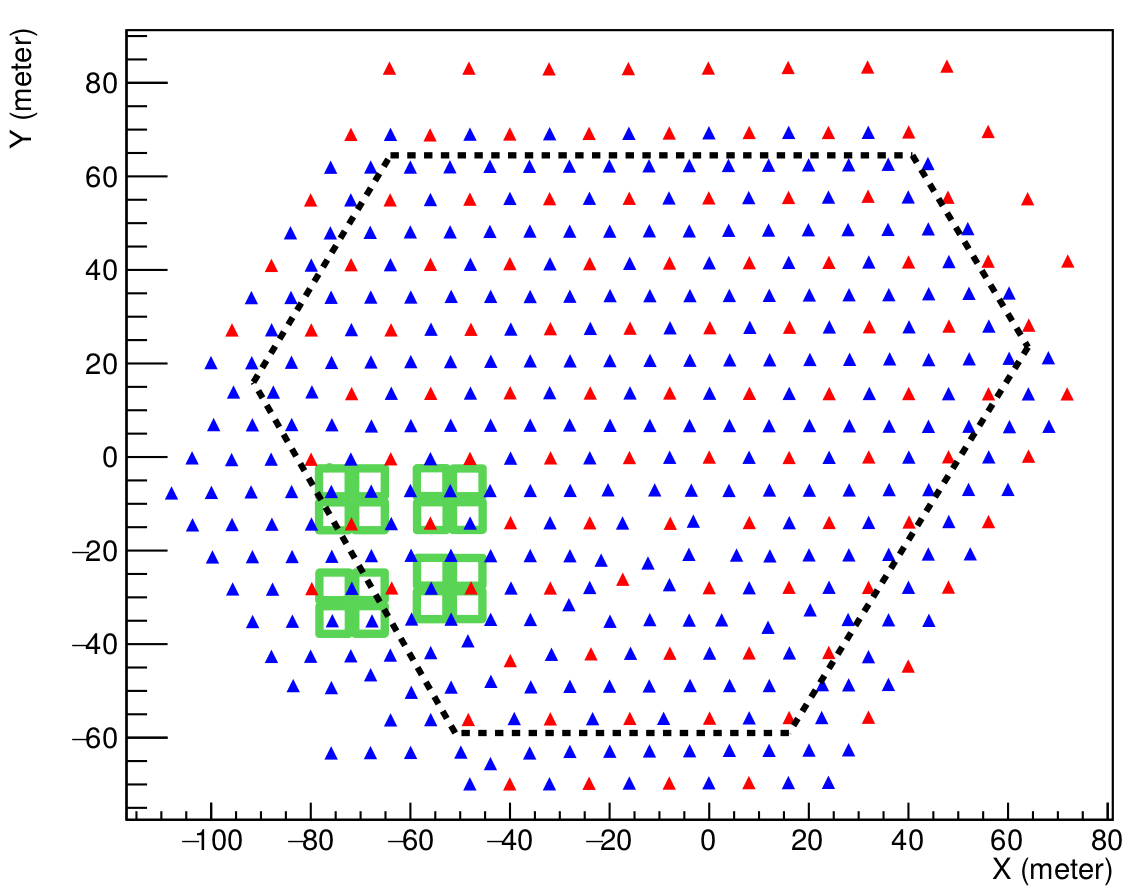
\includegraphics[width=0.9\linewidth, height=3.2cm]{array-map} 
\caption{Schematic of GRAPES-3 Detector Array}
\label{fig:array-map}
\end{subfigure}
\begin{subfigure}{0.245\textwidth}
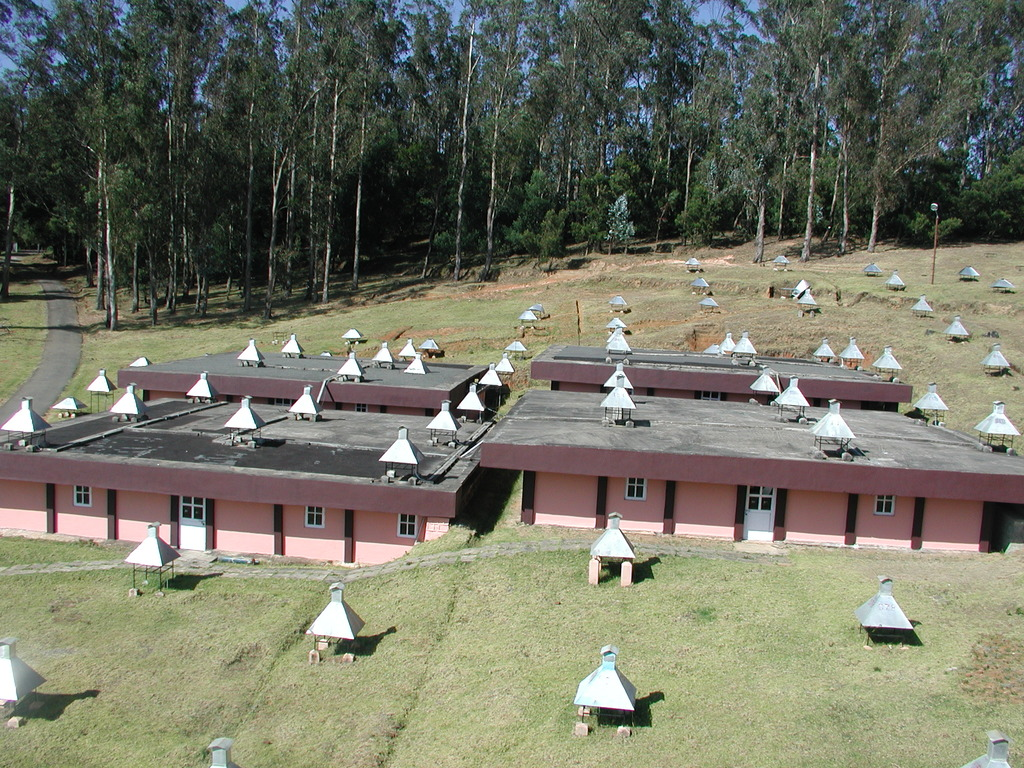
\includegraphics[width=0.9\linewidth, height=3cm]{detector} 
\caption{Scintillator detector and Muon station}
\label{fig:detector}
\end{subfigure}
\begin{subfigure}{0.245\textwidth}
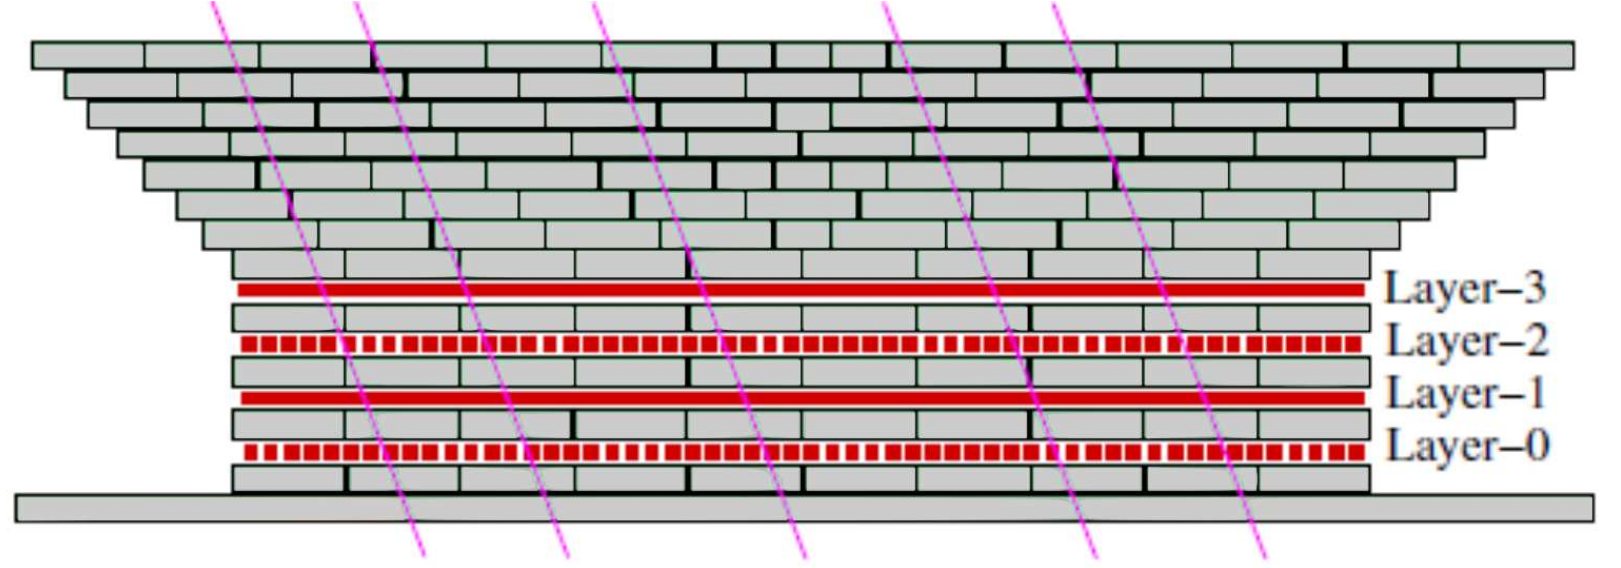
\includegraphics[width=0.9\linewidth, height = 3cm]{mu-station} 
\caption{Schematic of muon module}
\label{fig:mu-station}
\end{subfigure}
\begin{subfigure}{0.245\textwidth}
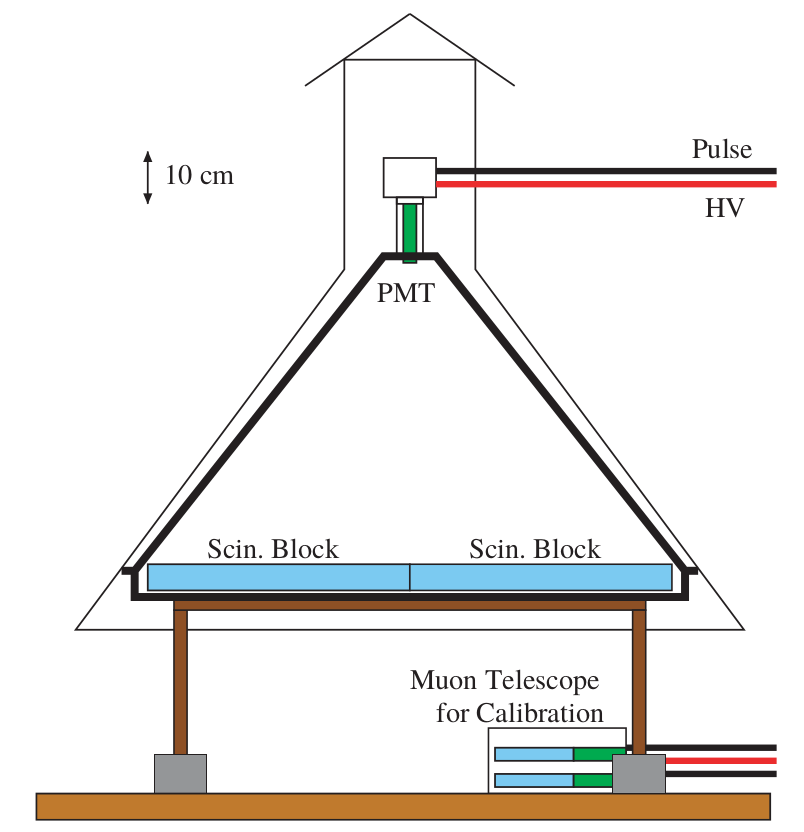
\includegraphics[width=0.9\linewidth, height = 3cm]{sc-detector}
\caption{Schematic of scintillator detector}
\label{fig:sc-detector}
\end{subfigure}
\caption{GRAPES-3 detector array}
\label{fig:g3array}
\end{figure}
 
The scintillator detectors (shown as filled triangles in Figure
\ref{fig:array-map}) are spread over an area of $\sim$25,000 m$^2$. Each of the
GRAPES-3 scintillator detector is 1 m$^2$ in area. The separation between two
scintillator detectors is 8 m, which makes it one of the most dense array among
the traditional EAS arrays. GRAPES-3 muon detector spread over an area of 560
m$^2$ is comprised of 16 closely packed modules (shown as squares in Figure
\ref{fig:array-map}). Each module contains 232 PRCs, placed in 4 layers,
arranged in orthogonal directions. Each layer consists of 58 PRCs kept closely
side by side. The effective area of each module is 35 m$^2$. This large area,
muon detector has been designed for studies on the composition of PCRs and
studies on cosmic sources of UHE $\gamma$-rays. Large area muon detector is
also required for observations on muons produced by lower energy protons which
are affected by phenomena occurring on the Sun, such as solar flares and
coronal mass ejections leading to magnetic disturbances around the Earth.

\section{Simulation of monoenergetic showers}

For the treatment of low energy hadronic interactions, two low energy hadronic
generators, namely FLUKA and GHEISHA, are commonly used. Table
\ref{tab:fluka-gheisha} shows the difference in muon multiplicity produced by
the two hadronic generators. Here, these are paired with SIBYLL2.3c and
QGSJETII-04 to treat high energy hadronic interactions. FLUKA combination gives
higher muon multiplicity as compared to GHEISHA combination. In the earlier
CORSIKA simulations, done for GRAPES-3 experiment, fluka was used as the low
energy hadronic generator. Hence, in this study also all the simulations were
done using FLUKA as low energy hadronic generator. 

\begin{table}
\centering
\begin{tabular}{ | c | c | c | c |} 
\hline
Model & Median & Sigma & Rel. S.D. (\%) \\ 
\hline
SIBYLL-GHEISHA &1161 & 273 & 23.5  \\ 
\hline
SIBYLL-FLUKA   & 1179 & 277 & 23.5  \\
\hline
QGSII-GHEISHA  & 1185 & 258 & 21.8  \\
\hline
QGSII-FLUKA  & 1200 & 250 & 20.8 \\
\hline
\end{tabular}
\caption{Comparison of muon  multiplicity distribution for a 100 TeV primary proton}
\label{tab:fluka-gheisha}
\end{table}

A comparison between the two Post-LHC hadronic interaction generators was done
to see the characteristics of the two generators. The comparison was done on
the basis of muon content produced by the two generators. The PCRs were assumed
to be composed of five species, protons (H, A = 1), helium (He, A = 4),
nitrogen (N, A = 14), aluminum (Al, A = 27) and iron (Fe, A = 56). Heavier
nuclei N, Al and Fe were used to represent light (C,N,O), medium (Mg, Al, Si)
and heavy (Mn, Fe, Co) masses in PCRs. For each primary, monoenergetic showers
with zenith angle $\theta$= 0$^{\circ}$ were simulated at energy: 10 TeV, 100
TeV, and 1000 TeV. Comparison of muon multiplicity was made: 1) between the
two generators, 2) between different primaries for each generator.

Since the threshold energy of muon telescope of GRAPES-3 experiment is
1$\times$Sec($\theta$) GeV, where $\theta$ is the zenith angle of muon, in
simulations also, the muons with energy greater than 1$\times$sec($\theta$) GeV
were counted. Table \ref{tab:muon_multiplicity} shows the variation of median
muon multiplicity with changing primaries, primary energies, and with different
generators. 

\begin{table}
\centering
%\begin{tabular}{ | p{1.5cm} | p{2cm} | p{1.5cm} | p{2cm} | p{1.5cm} |} 
\begin{tabular}{ | c | c | c | c | c | c |} 
\hline
& \multicolumn{2}{|c|}{\textbf{SIBYLL-FLUKA}} & \multicolumn{2}{|c|}{\textbf{QGSJETII-FLUKA}} & S vs Q \\
\hline
 & Median & \% Increase & Median & \% Increase & \% Increase \\
\hline 
\multicolumn{6}{|c|}{\textbf{10 TeV}} \\
\hline
H 	&	146	&	      & 150 &			& 2.7 \\
\hline
He 	&	174 &	19.2 &	182	&	21.33	&	4.6	\\
\hline
N 	& 	214 & 	46.6 &	227	&	51.33	&6.0	\\
\hline
Al 	& 	239 & 	63.7 &	254	&	69.33	&6.3	\\
\hline
Fe 	& 	259 & 	77.4 &	278	&	85.33	&7.3	\\
\hline
\multicolumn{6}{|c|}{\textbf{100 TeV}} \\
\hline
H & 1180 &  & 1200 & & 1.7 \\
\hline
He & 1340 & 13.6  & 1375 & 14.58	& 2.6\\
\hline
N & 1531 & 29.8 & 1577 & 31.42 	& 3.0\\
\hline
Al & 1659 & 40.6 & 1724 & 43.67 	& 3.9\\
\hline
Fe & 1845 & 56.4 & 1931 & 60.92	& 4.7\\
\hline
\multicolumn{6}{|c|}{\textbf{1000 TeV}} \\
\hline
H & 9393 &  & 9586 & & 2.1\\
\hline
N & 12132 & 29.2 & 12337 & 28.7 & 1.7\\
\hline
Fe & 13874 & 47.7 & 14284 & 49.0 & 3.0\\
\hline
\end{tabular}
\caption{Median muon multiplicity at 10 TeV, 100 TeV, and 1000 TeV. Column 3 and 5 show the percentage increase in muon multiplicity of different primaries w.r.t. H of respective generators. Column "S vs Q" shows the percentage increase in muon multiplicity in QGSJETII-FLUKA w.r.t. that of SIBYLL-FLUKA.\label{tab:muon_multiplicity}}
\end{table}

Table \ref{tab:muon_multiplicity} shows that QGSJETII-FLUKA gives slightly
	higher muon multiplicity as compared to SIBYLL-FLUKA and the difference
	increases with mass of primary. As the energy increases from 10 TeV to
	1000 TeV, the difference in muon multiplicity of two generators
	decrease. Figure \ref{fig:sibyllmm} and Figure \ref{fig:qgsiimm} show
	the muon multiplicity distributions  at different primary energies.

\begin{figure}
\begin{subfigure}{0.32\textwidth}
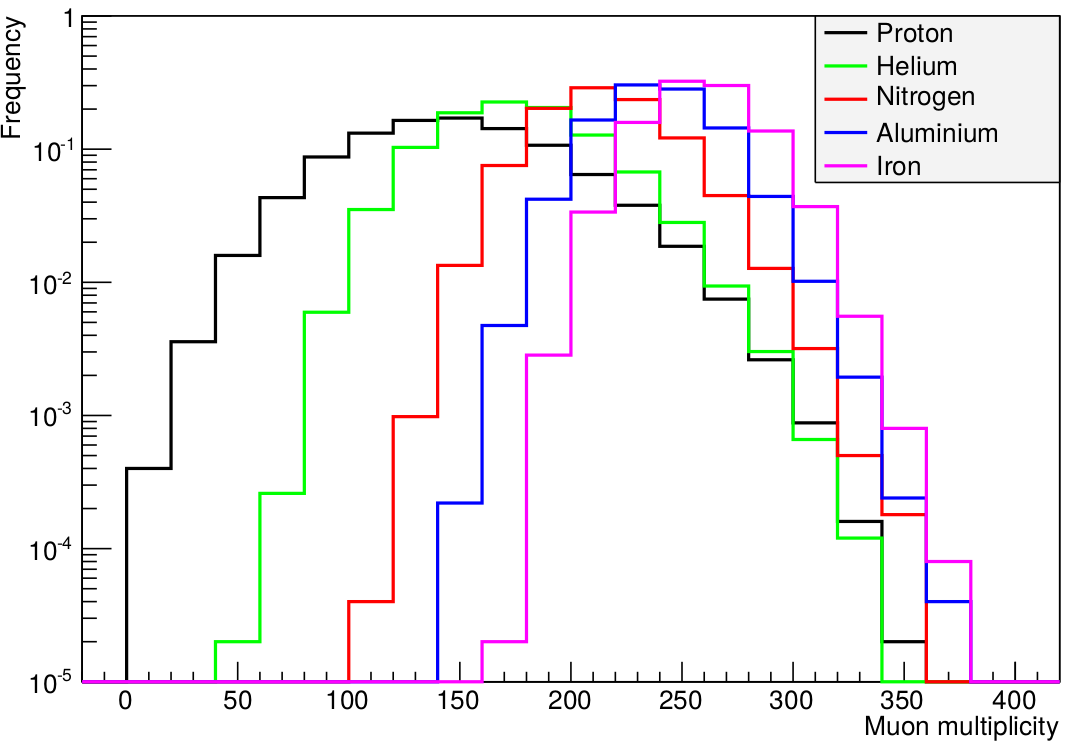
\includegraphics[width=0.9\linewidth, height=3cm]{sibyllmm10} 
\caption{10 TeV}
\label{fig:sibyllmm10}
\end{subfigure}
\begin{subfigure}{0.32\textwidth}
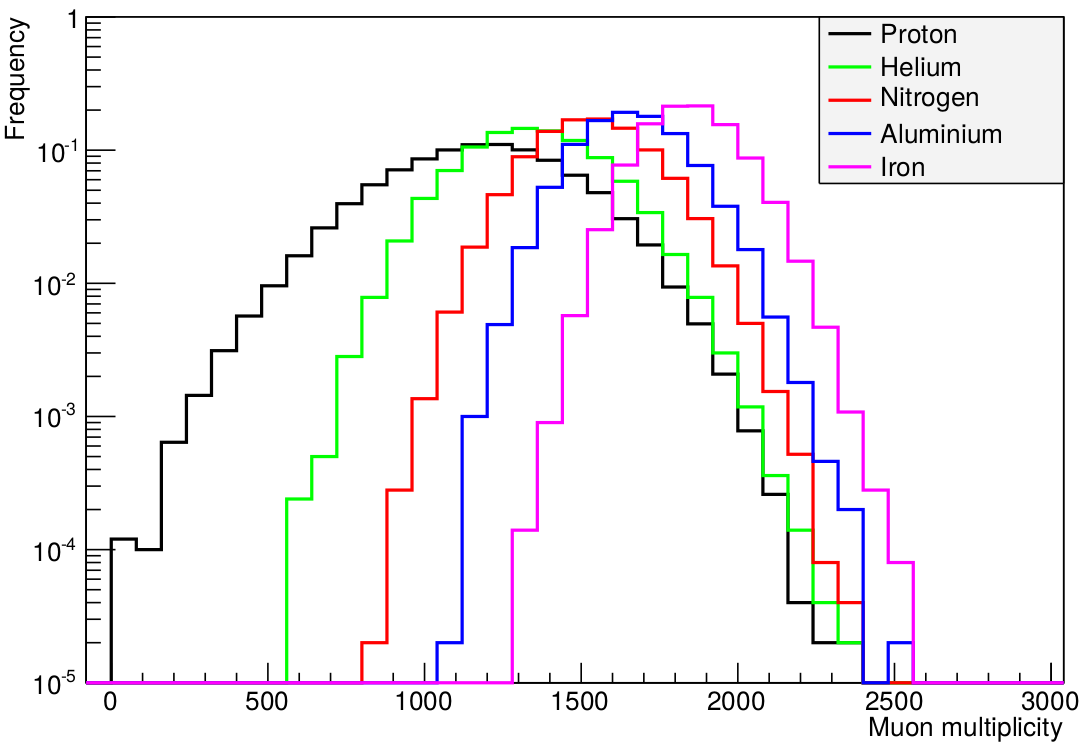
\includegraphics[width=0.9\linewidth, height=3cm]{sibyllmm100} 
\caption{100 TeV}
\label{fig:sibyllmm100}
\end{subfigure}
\begin{subfigure}{0.32\textwidth}
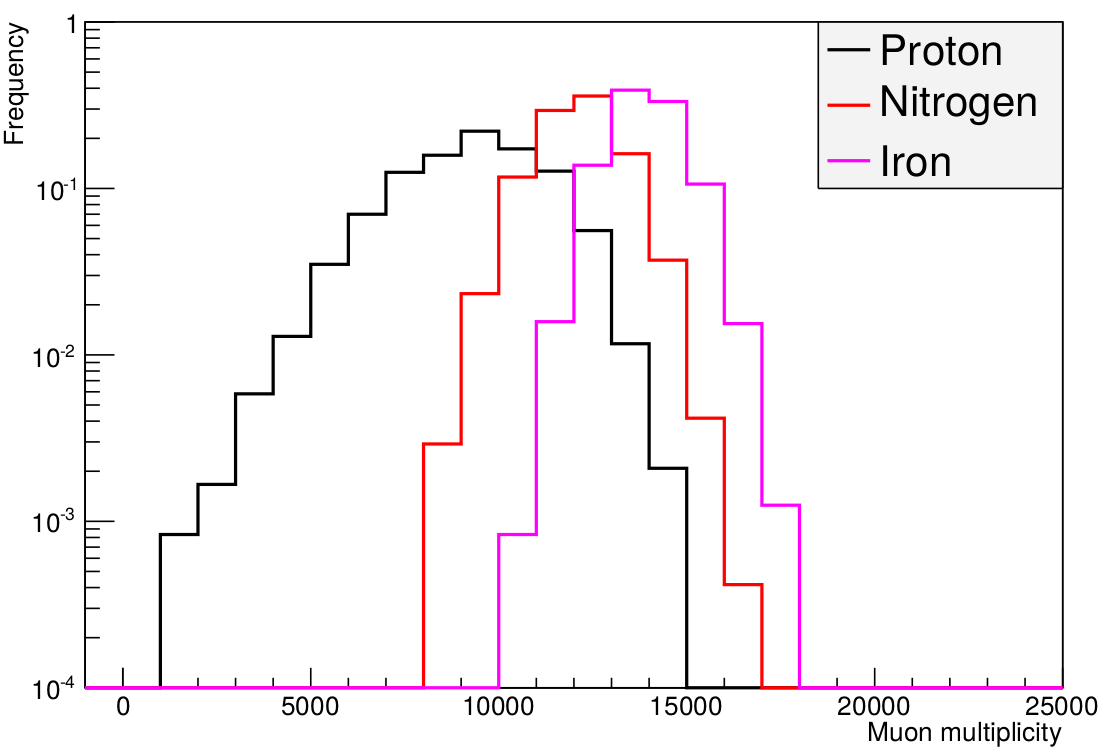
\includegraphics[width=0.9\linewidth, height = 3cm]{sibyllmm1000} 
\caption{1000 TeV}
\label{fig:sibyllmm1000}
\end{subfigure}
\caption{Muon multiplicity distribution for different primaries using SIBYLL-FLUKA}
\label{fig:sibyllmm}
\end{figure}
 

\begin{figure}
\begin{subfigure}{0.32\textwidth}
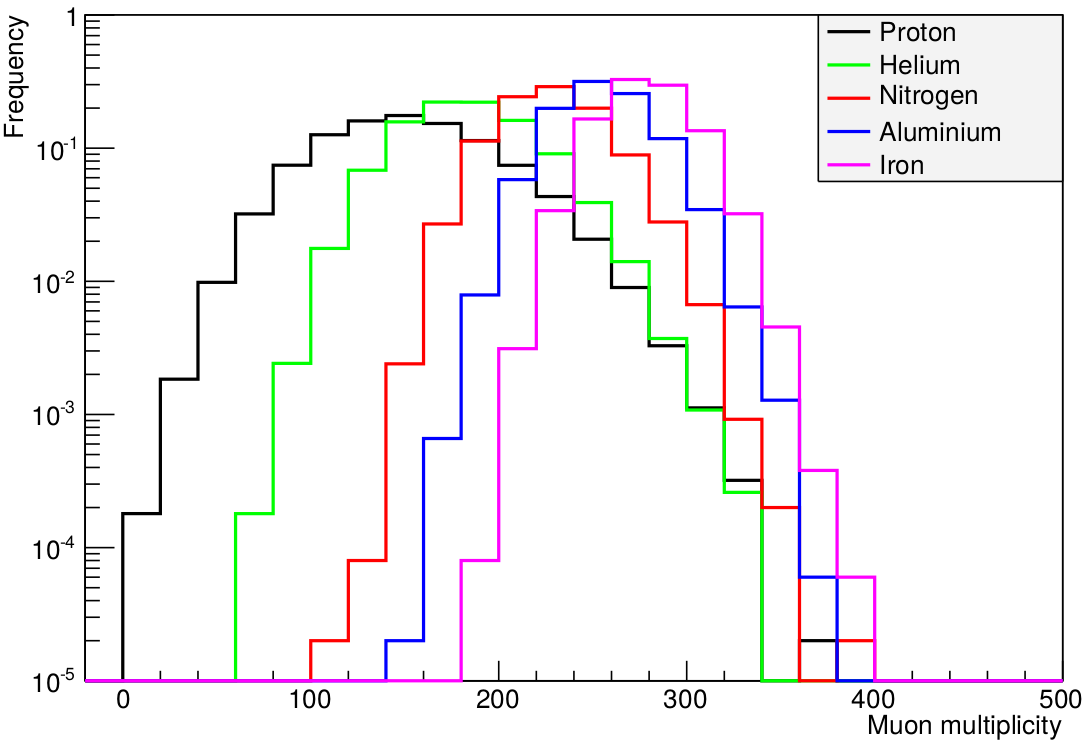
\includegraphics[width=0.9\linewidth, height=3cm]{qgsiimm10} 
\caption{10 TeV}
\label{fig:qgsiimm10}
\end{subfigure}
\begin{subfigure}{0.32\textwidth}
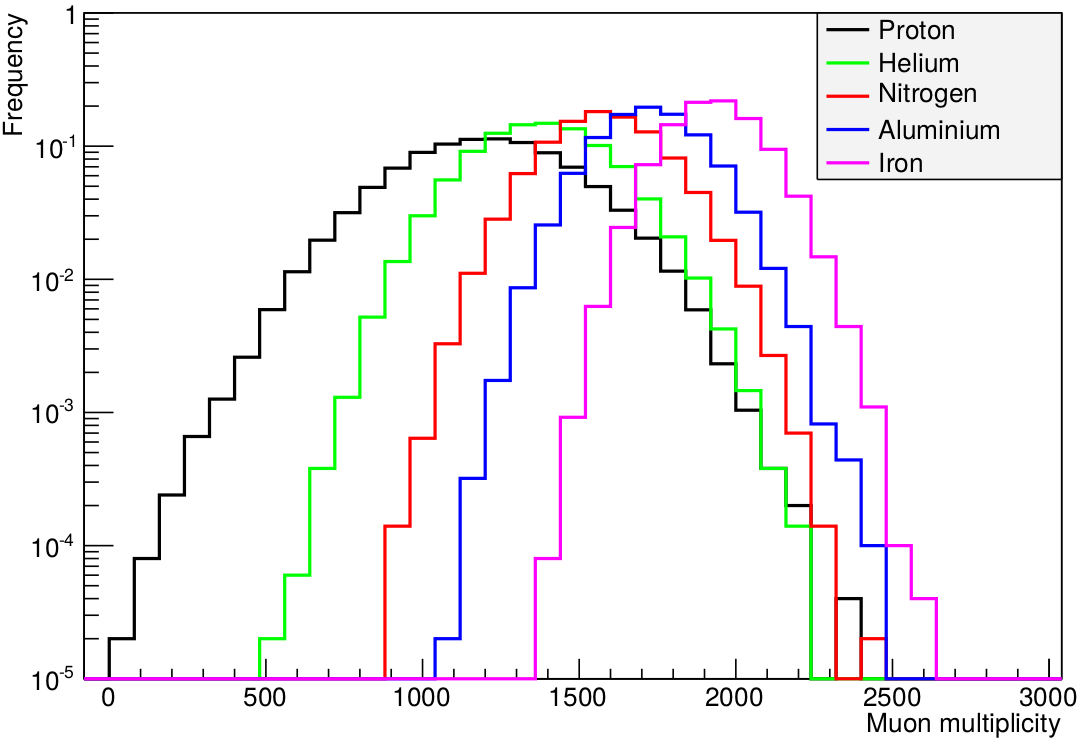
\includegraphics[width=0.9\linewidth, height=3cm]{qgsiimm100} 
\caption{100 TeV}
\label{fig:qgsiimm100}
\end{subfigure}
\begin{subfigure}{0.32\textwidth}
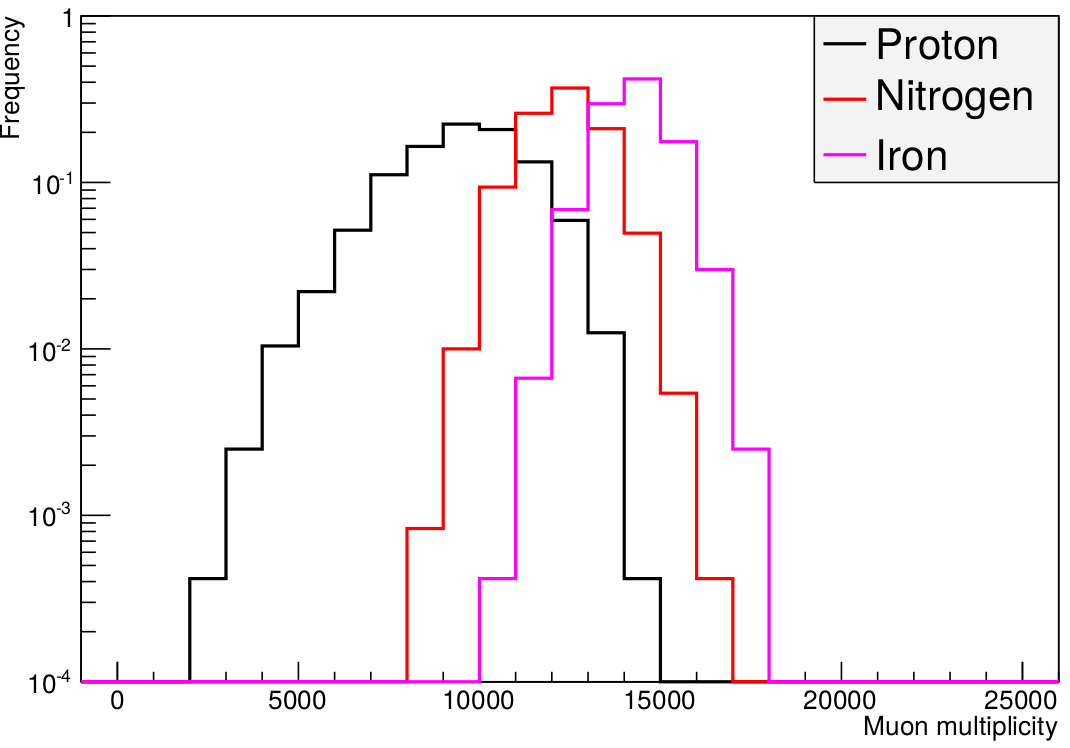
\includegraphics[width=0.9\linewidth, height = 3cm]{qgsiimm1000} 
\caption{1000 TeV}
\label{fig:qgsiimm1000}
\end{subfigure}
\caption{Muon multiplicity distribution for different primaries using QGSJETII-FLUKA}
\label{fig:qgsiimm}
\end{figure}


Monoenergeric proton induced showers with zenith angle = 0$^\circ$ were
simulated using generators of CORSIKA-6.99, namely SIBYLL 2.1 and QGSJETII-03,
at energies: 10 TeV, 100 TeV, and 1000 TeV. Table
\ref{tab:muon_multiplicity_lhc} shows that the difference between median muon
multiplicity of SIBYLL- and QGSJETII-FLUKA is more in pre-LHC as compared to
post-LHC generators. In other words, the post-LHC generators are expected to
give relatively close results in shower analysis as compared to pre-LHC
generators. Column 3 and column 5 of the Table \ref{tab:muon_multiplicity_lhc}
show that the difference of median muon multiplicity between pre- and post-LHC
generators is higher for more massive primaries. 


\begin{table}
\centering
\begin{tabular}{ | c | c | c | c | c | c |} 
\hline
& \multicolumn{2}{|c|}{\textbf{SIBYLL-FLUKA}} & \multicolumn{2}{|c|}{\textbf{QGSJETII-FLUKA}} & S vs Q \\
\hline
 & Median & \% Increase & Median & \% Increase & \% Increase \\
\hline 
\multicolumn{6}{|c|}{\textbf{10 TeV}} \\
\hline
Pre-LHC 	&	130	&	      & 142 &			& 9.2 \\
\hline
Post-LHC 	&	146	&	12.3      & 150 &	5.6		& 2.7 \\
\hline
\multicolumn{6}{|c|}{\textbf{100 TeV}} \\
\hline
Pre-LHC & 1006 &  & 1088 & & 8.2 \\
\hline
Post-LHC & 1180 & 17.3 & 1200 & 10.3 & 1.7 \\
\hline
\multicolumn{6}{|c|}{\textbf{1000 TeV}} \\
\hline
Pre-LHC & 7866 &  & 8327 & & 5.9\\
\hline
Post-LHC & 9393 & 19.4 & 9586 & 15.1 & 2.1\\
\hline
\end{tabular}
\caption{Median muon multiplicity at 10 TeV, 100 TeV, and 1000 TeV using Pre-LHC and Post-LHC generators. Column 3 and 5 represents the percentage increase in muon multiplicity of Post-LHC hadronic generators w.r.t. that of Pre-LHC hadronic generators. Column 6 represents the percentage increase in muon multiplicity in QGSJETII-FLUKA w.r.t. that of SIBYLL-FLUKA.\label{tab:muon_multiplicity_lhc}}
\end{table}

\begin{figure}
\begin{subfigure}{0.32\textwidth}
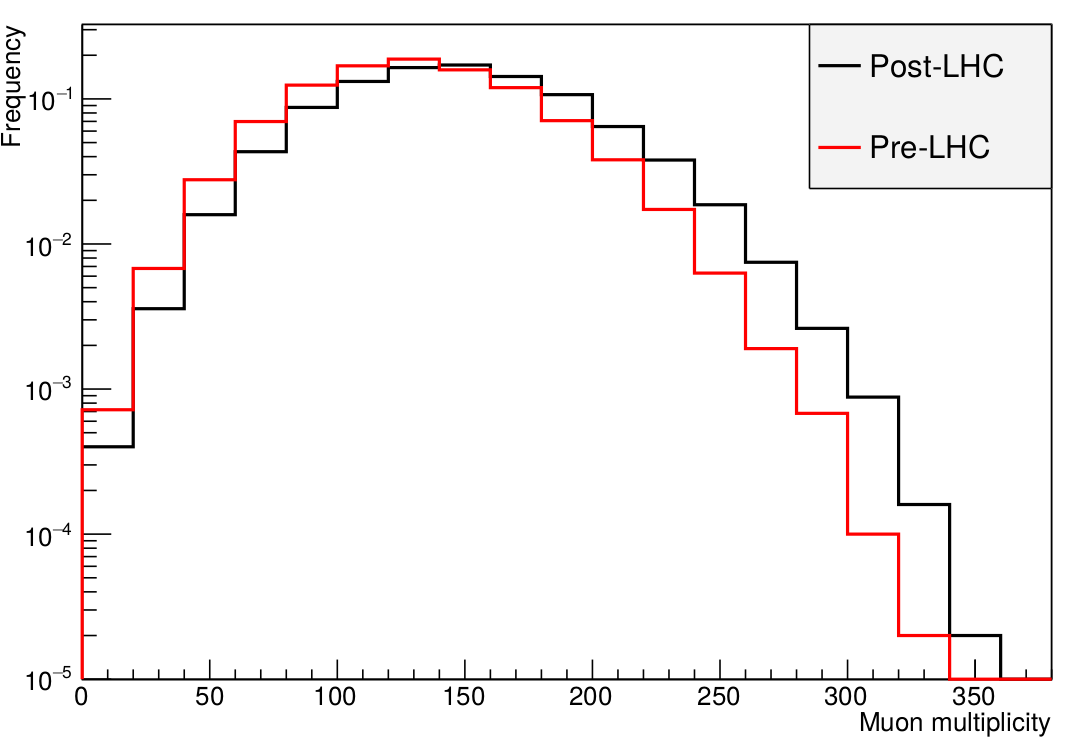
\includegraphics[width=0.9\linewidth, height=3cm]{sibyll-lhc-mm10} 
\caption{10 TeV}
\label{fig:sibyll-lhc-mm10}
\end{subfigure}
\begin{subfigure}{0.32\textwidth}
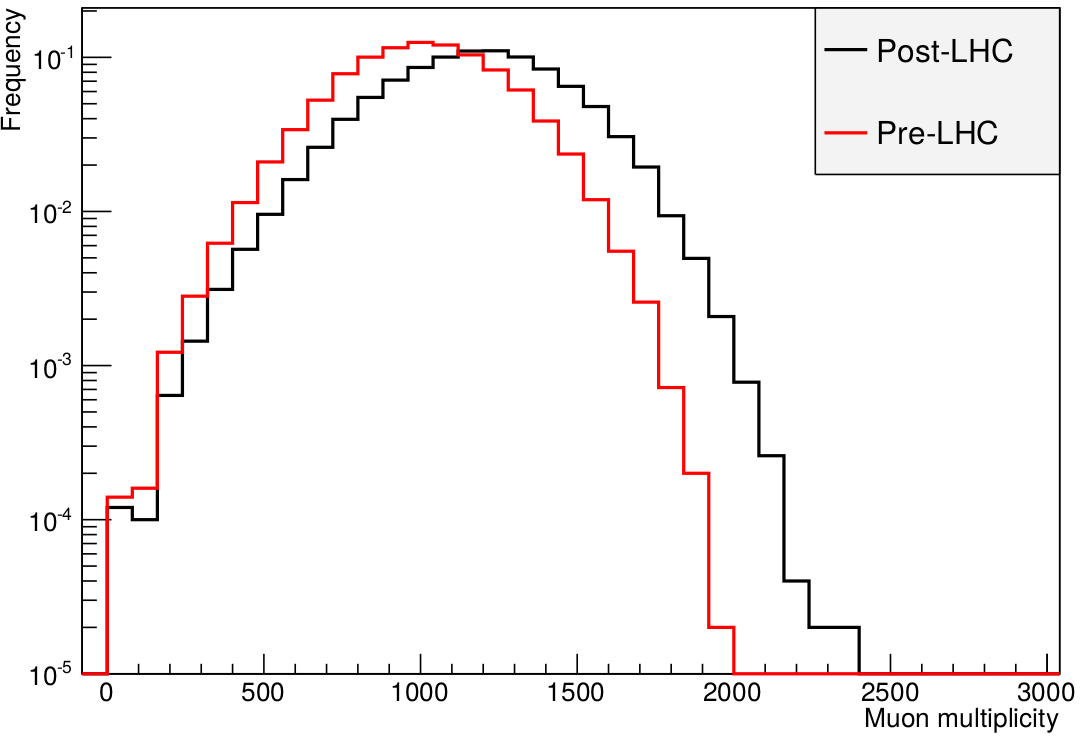
\includegraphics[width=0.9\linewidth, height=3cm]{sibyll-lhc-mm100} 
\caption{100 TeV}
\label{fig:sibyll-lhc-mm100}
\end{subfigure}
\begin{subfigure}{0.32\textwidth}
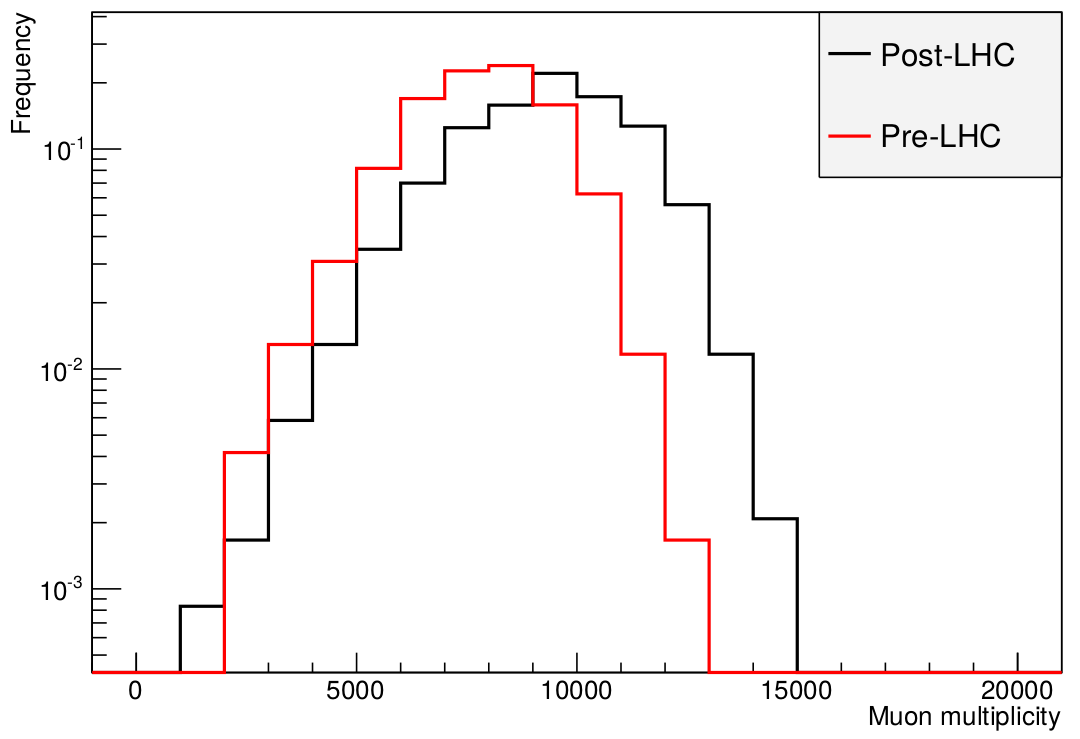
\includegraphics[width=0.9\linewidth, height = 3cm]{sibyll-lhc-mm1000} 
\caption{1000 TeV}
\label{fig:sibyll-lhc-mm1000}
\end{subfigure}
\caption{Muon multiplicity distribution of Pre- and Post-LHC hadronic generators using SIBYLL-FLUKA}
\label{fig:lhc_multiplicity_sibyll}
\end{figure}



\begin{figure}
\begin{subfigure}{0.32\textwidth}
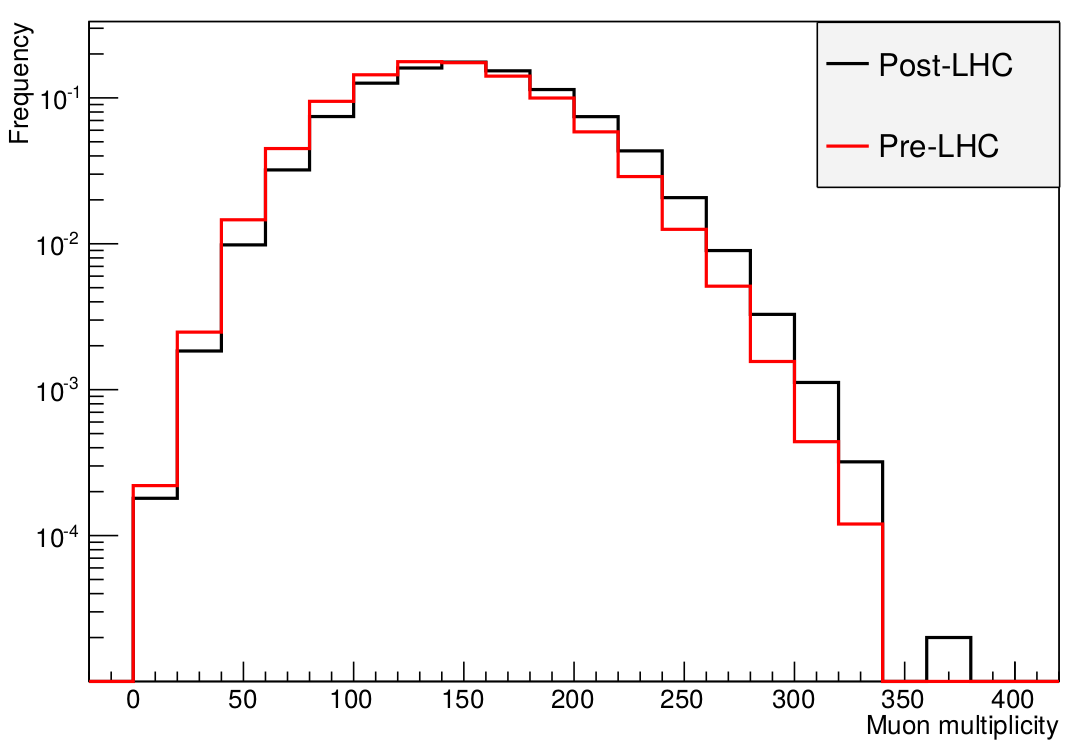
\includegraphics[width=0.9\linewidth, height=3cm]{qgsii-lhc-mm10} 
\caption{10 TeV}
\label{fig:qgsii-lhc-mm10}
\end{subfigure}
\begin{subfigure}{0.32\textwidth}
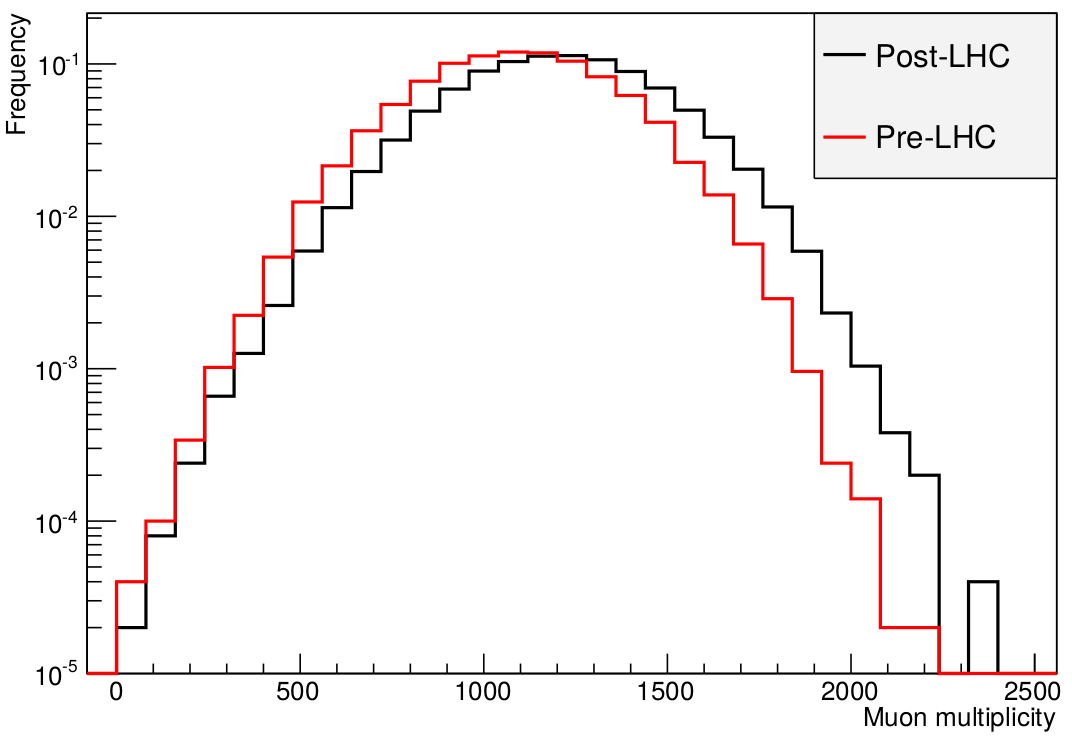
\includegraphics[width=0.9\linewidth, height=3cm]{qgsii-lhc-mm100} 
\caption{100 TeV}
\label{fig:qgsii-lhc-mm100}
\end{subfigure}
\begin{subfigure}{0.32\textwidth}
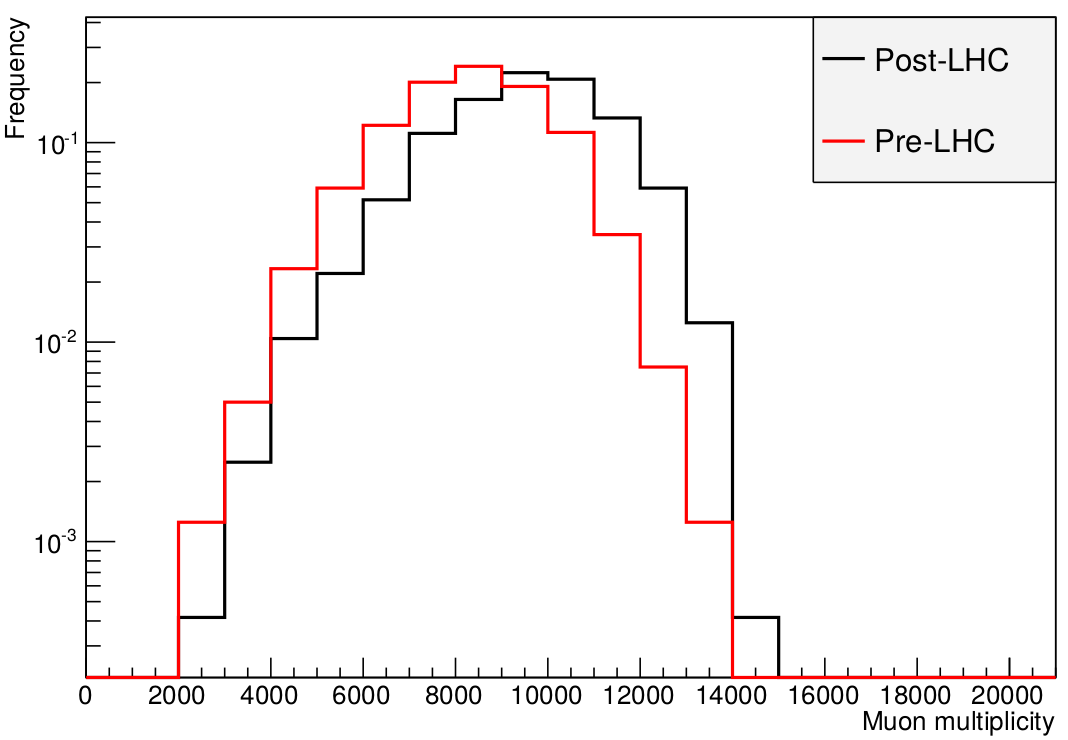
\includegraphics[width=0.9\linewidth, height = 3cm]{qgsii-lhc-mm1000} 
\caption{1000 TeV}
\label{fig:qgsii-lhc-mm1000}
\end{subfigure}
\caption{Muon multiplicity distribution of Pre- and Post-LHC hadronic generators using QGSJETII-FLUKA}
\label{fig:lhc_multiplicity_qgsii}
\end{figure}

\section{Comparison of simulations with GRAPES-3 data}

The long-term aim of this study is to find the mass composition of cosmic rays
by analyzing the shower data in the energy range $\sim$100 TeV to $\sim$1000
TeV. A similar study was done earlier by Tanaka et al. by using CORSIKA-6.02's
hadronic generators SIBYLL-2.1 and QGSJET-01 as high energy hadronic generators
and GHEISHA as low energy hadronic generator. Both of the high energy hadronic
generators had parameters which were not tuned with LHC data, hence these
generators were Pre-LHC generators. Tanaka et al. simulated the showers in the
energy range of 100 TeV - 1000 TeV with the following primaries: H, He, N, Al,
and Fe. Figure \ref{fig:tanaka_spectrum} shows the muon multiplicity plot of
experimental data (dots) and weighted sum of contributions due to all the
primaries for $N_e = 10^{5.0}$ and $10^{5.2}$. The idea was to fit the
multiplicity data of primaries to the experimental data and relate the
weighting fractions of different primaries to their relative abundance. But the
difference in the composition gven by the two generators was significantly
large. Table \ref{tab:muon_multiplicity_lhc}, shows that the difference between
the muon multiplicity of SIBYLL-FLUKA and QGSJETII-FLUKA is less in case of
post LHC generators as compared to pre-LHC generators. Therefore, we expect the
two post-LHC generators to give similar results in the spectrum data analysis.
\linebreak




\begin{thebibliography}{9}
 
\bibitem{raghu} R A Shukla, V G Achanta, P D Barbaro, S R Dugad, A Heering, S K Gupta, I Mirza, S S Prabhu, P Rumerio, "Microscopic Characterisation of Photo Detectors from CMS Hadron Calorimeter".
arXiv:1806.09887 [physics.ins-det].
  
\end{thebibliography}

 

\end{document}

